\fontfamily{\sfdefault}\selectfont
% XCircuit output "discrete_pll_full_noise.tex" for LaTeX input from discrete_pll_full_noise.ps
\def\putbox#1#2#3#4{\makebox[0.00000in][l]{\makebox[#1][l]{}\raisebox{\baselineskip}[0.00000in][0.00000in]{\raisebox{#2}[0.00000in][0.00000in]{\scalebox{#3}{#4}}}}}
\def\rightbox#1{\makebox[0.00000in][r]{#1}}
\def\centbox#1{\makebox[0.00000in]{#1}}
\def\topbox#1{\raisebox{-0.60\baselineskip}[0.00000in][0.00000in]{#1}}
\def\midbox#1{\raisebox{-0.20\baselineskip}[0.00000in][0.00000in]{#1}}
   \scalebox{1}{
   \normalsize
   \parbox{6.30000in}{
   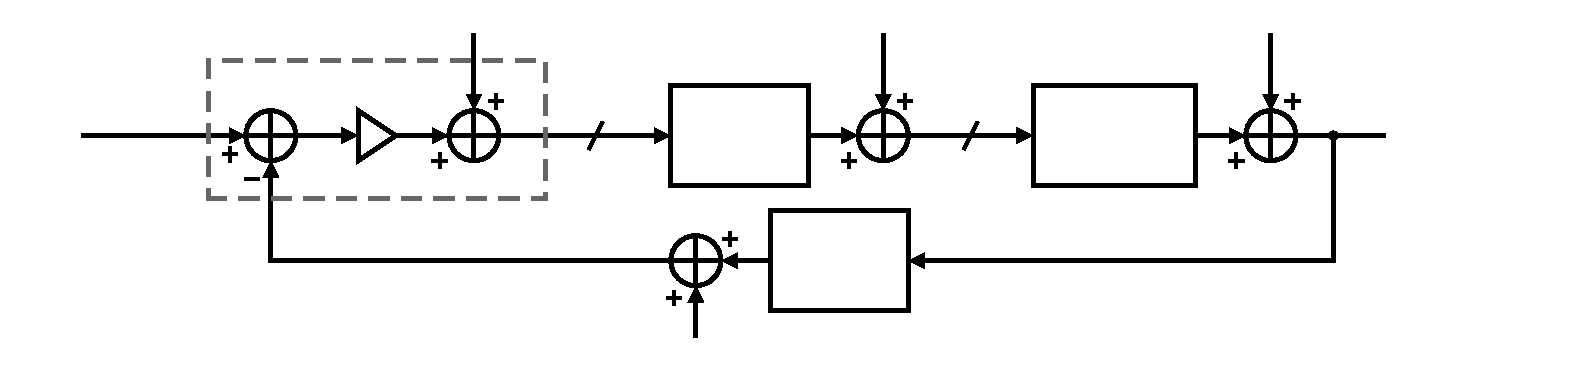
\includegraphics[scale=0.60000]{./figs/discrete_pll_full_noise.pdf}\\
   % translate x=416 y=544 scale 0.38
   \putbox{0.33600in}{1.00800in}{0.84}{$\Phi_{ref}$(t)}%
   \putbox{1.56000in}{0.51000in}{0.84}{$\Phi_{div}$(t)}%
   \putbox{2.27400in}{1.03200in}{0.84}{e$_\Phi$(t)}%
   \putbox{1.42200in}{1.08600in}{0.84}{\rotatebox{-360}{$K_{PD}$}}%
   \putbox{1.20600in}{1.00800in}{0.84}{$\Phi_e$}%
   \putbox{0.83400in}{1.28400in}{0.84}{PD}%
   \putbox{2.77200in}{0.89400in}{0.84}{H$_{LF}$(s)}%
   \putbox{3.79800in}{1.02000in}{0.84}{u(t)}%
   \putbox{4.26000in}{0.90600in}{0.84}{$\frac{2\pi K_{DCO}}{s}$}%
   \putbox{5.22000in}{0.99600in}{0.84}{$\Phi_{out}$(t)}%
   \putbox{3.22200in}{0.39600in}{0.84}{$\div$ N}%
   \putbox{4.13400in}{1.17000in}{0.84}{DCO}%
   \putbox{1.93200in}{1.30800in}{0.84}{q$_{n_{PD}}$(t)}%
   \putbox{3.57000in}{1.30800in}{0.84}{\rotatebox{-360}{q$_{n_{LF}}$(t)}}%
   \putbox{2.82000in}{0.09600in}{0.84}{$\Phi_{n_{div}}$(t)}%
   \putbox{5.12400in}{1.30800in}{0.84}{$\Phi_{n_{DCO}}$(t)}%
   } % close 'parbox'
   } % close 'scalebox'
   \vspace{-\baselineskip} % this is not necessary, but looks better
\fontfamily{\rmdefault}\selectfont
